\documentclass[../main.tex]{subfiles}
\begin{document}
\chapter{Bit Manipulation}
Many books on algorithmic problem solving seems forget about one topic--bit and bit manipulation. Bit is how data is represented and saved on the hardware. Thus knowing such concept and bit manipulation using Python sometimes can also help us device more efficient algorithms, either space or time complexity in the later Chapter. 


For example, how to convert a char or integer to bit, how to get each bit, set each bit, and clear each bit. Also, some more advanced bit manipulation operations. After this, we will see some examples to show how to apply bit manipulation in real-life problems. 
%%%%%%%%%%%%%%%%%%%%%%Bit operators%%%%%%%%%%%%
\section{Python Bitwise Operators}
\label{sec_basic_bit_operator}
Bitwise operators include <<, >>, \&, |, \~, \^. All of these operators operate on signed or unsigned numbers, but instead of treating that number as if it were a single value, they treat it as if it were a string of bits. Twos-complement binary is used for representing the singed number.  




Now, we introduce the six bitwise operators.
\paragraph{x \texttt{<<} y} Returns $x$ with the bits shifted to the left by $y$ places (and new bits on the right-hand-side are zeros). This is the same as multiplying $x$ by $2^y$.

\paragraph{x \texttt{>>} y} Returns $x$ with the bits shifted to the right by $y$ places. This is the same as dividing $x$ by $2^y$, same result as the $//$ operator. This right shift is also called \textit{arithmetic right shift}, it fills in the new bits with the value of the sign bit. 

\paragraph{x \texttt{\&} y} "Bitwise and". Each bit of the output is 1 if the corresponding bit of $x$ AND of $y$ is 1, otherwise it's 0. It has the following property: 
\begin{lstlisting}[language=Python]
# keep 1 or 0 the same as original
1 & 1 = 1
0 & 1 = 0
# set to 0 with & 0
1 & 0 = 0
0 & 0 = 0
\end{lstlisting}

\paragraph{x \texttt{|} y} "Bitwise or".  Each bit of the output is 0 if the corresponding bit of $x$ AND of $y$ is 0, otherwise it's 1.
\begin{lstlisting}[language=Python]
# set to 1 with | 1
1 | 1 = 1
0 | 1 = 1

# keep 1 or 0 the same as original
1 | 0 = 1
0 | 0 = 0
\end{lstlisting}

\paragraph{$\thicksim x
$} Returns the complement of x - the number you get by switching each 1 for a 0 and each 0 for a 1. This is the same as $-x - 1$(really?). 

\paragraph{x $\wedge$ y} "Bitwise exclusive or". Each bit of the output is the same as the corresponding bit in $x$ if that bit in $y$ is 0, and it's the complement of the bit in $x$ if that bit in $y$ is 1. It has the following basic properties:
\begin{lstlisting}[language=Python]
# toggle 1 or 0 with ^ 1
1 ^ 1 = 0
0 ^ 1 = 1

# keep 1 or 0 with ^ 0
1 ^ 0 = 1
0 ^ 0 = 0
\end{lstlisting}
Some examples shown: 
\begin{lstlisting}
A = 5 = 0101, B = 3 = 0011
 A ^ B = 0101 ^ 0011 = 0110 = 6
 \end{lstlisting}
More advanced properties of XOR operator include:
 \begin{lstlisting}
a ^ b = c 
c ^ b = a

n ^ n = 0
n ^ 0 = n
eg. a=00111011, b=10100000 , c= 10011011, c ^b= a
 \end{lstlisting}

\paragraph{Logical right shift} The logical right shift is different to the above right shift after shifting it puts a 0 in the most significant bit. It is indicated with a $>>>$ operator n Java. However, in Python, there is no such operator, but we can implement one easily using \textbf{bitstring} module padding with zeros using $>>=$ operator.
\begin{lstlisting}[language=Python]
>>> a = BitArray(int=-1000, length=32)
>>> a.int
-1000
>>> a >>= 3
>>> a.int
536870787
\end{lstlisting}

%%%%%%%%%%%%%%%%%%%%%%%Useful Python function%%%%%%%%%%%%%%%%%%%%
\section{Python Built-in Functions}
\label{sec_bitwise_built_in_function}
\paragraph{bin()} The bin() method takes a single parameter \textbf{num}- an integer and return its \textit{binary string}. If not an integer, it raises a TypeError exception. 
\begin{lstlisting}[language=Python]
a = bin(88)
print(a)
# output
# 0b1011000
\end{lstlisting}
However, bin() doesn't return \textit{binary bits} that applies the two's complement rule. For example, for the negative value:
\begin{lstlisting}[language=Python]
a1 = bin(-88)
# output
# -0b1011000
\end{lstlisting}
\paragraph{int(x, base = 10)} The int() method takes either a string x  to return an integer with its corresponding base. The common base are: 2, 10, 16 (hex). 
\begin{lstlisting}[language=Python]
b = int('01011000', 2)
c = int('88', 10)
print(b, c)
# output
# 88 88
\end{lstlisting}

\paragraph{chr()} The chr() method takes a single parameter of integer and return a character (a string) whose Unicode code point is the integer. If the integer i is outside the range, ValueError will be raised.
\begin{lstlisting}[language=Python]
d = chr(88)
print(d)
# output
# X
\end{lstlisting}
\paragraph{ord()} The ord() method takes a string representing one Unicode character and return an integer representing the Unicode code point of that character. 
\begin{lstlisting}[language=Python]
e = ord('a')
print(e)
# output
#  97
\end{lstlisting}

%%%%%%%%%%%%%%%%Two's complement Binary%%%%%%%%%%%%%%%%%%%%%%
\section{Twos-complement Binary} 
Given 8 bits, if it is unsigned, it can represent the values 0 to 255 (1111,1111). However, a two's complement 8-bit number can only represent positive integers from 0 to 127 (0111,1111) because the most significant bit is used as sign bit: '0' for positive, and '1' for negative. 
\begin{equation}
  \sum_{i=0}^{N-1} 2^i =  2^{(N-1)}+2^{(N-2)}+...+2^2+2^1+2^0= 2^N-1
\end{equation}
The twos-complement binary is the same as the classical binary representation for positive integers and differs slightly for negative integers. Negative integers are represented by performing Two's complement operation on its absolute value: it would be $(2^N-n)$ for representing $-n$ with N-bits. 
Here, we show Two's complement binary for eight-bit signed integers in Fig.~\ref{fig:twos_complement}.  
\begin{figure}
    \centering
    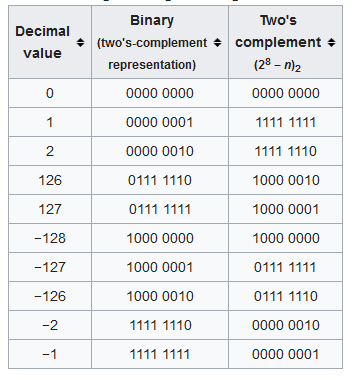
\includegraphics[width=0.6\columnwidth]{fig/eight_bit_two_complement.png}
    \caption{Two's Complement Binary for Eight-bit Signed Integers.}
    \label{fig:twos_complement}
\end{figure}
\paragraph{Get Two's Complement Binary Representation}
In Python, to get the two's complement binary representation of a given integer, we do not really have a built-in function to do it directly for negative number. Therefore, if we want to know how the two's complement binary look like for negative integer we need to write code ourselves. The Python code is given as:
\begin{lstlisting}[language=Python]
bits = 8
ans = (1 << bits) -2
print(ans)
# output
# '0b11111110'
\end{lstlisting}
There is another method to compute: inverting the bits of n (this is called \textbf{One's Complement}) and adding 1. For instance, use 8 bits integer 5, we compute it as the follows:
\begin{align}
\label{five}
    5_{10} &= {0000, 0101}_2, \\
    {-5}_{10} &= {1111, 1010}_2 + 1_2, \\ 
    {-5}_{10} &= {1111, 1011}_2
\label{five_complement}
\end{align}
To flip a binary representation, we need expression x XOR '1111,1111', which is $2^N-1$. The Python Code is given:
\begin{lstlisting}[language=Python]
def twos_complement(val, bits):
    # first flip implemented with xor of val with all 1's
    flip_val = val ^ (1 << bits - 1)
    #flip_val = ~val we only give 3 bits
    return bin(flip_val + 1)
\end{lstlisting}

\paragraph{Get Two's Complement Binary Result}
In Python, if we do not want to see its binary representation but just the result of two's complement of a given positive or negative integer, we can use two operations $-x$ or $\thicksim +1$. For input 2, the output just be a negative integer -2 instead of its binary representation:
\begin{lstlisting}[language=Python]
def twos_complement_result(x):
    ans1 = -x
    ans2 = ~x + 1
    print(ans1, ans2)
    print(bin(ans1), bin(ans2))
    return ans1
# output
# -8 -8
# -0b1000 -0b1000
\end{lstlisting}
This is helpful if we just need two's complement result instead of getting the binary representation. 


%%%%%%%%%%%%%%%%%%%%%%%Useful operation%%%%%%%%%%%%%%%%%%%%
\section{Useful Combined Bit Operations}
\label{sec_useful_bit_combination}

For operations that handle each bit, we first need a \textit{mask} that only set that bit to 1 and all the others to 0, this can be implemented with arithmetic left shift sign by shifting 1 with 0 to n-1 steps for n bits: 
\begin{lstlisting}[language=Python]
mask = 1 << i
\end{lstlisting}
\paragraph{Get ith Bit} In order to do this, we use the property of AND operator either 0 or 1 and with 1, the output is the same as original, while if it is and with 0, they others are set with 0s.
\begin{lstlisting}[language=Python]
# for n bit, i in range [0,n-1]
def get_bit(x, i):
    mask = 1 << i
    if x & mask:
        return 1
    return 0
print(get_bit(5,1))
# output 
# 0
\end{lstlisting}
Else, we can use left shift by i on x, and use AND with a single 1.
\begin{lstlisting}[language=Python]
def get_bit2(x, i):
    return x >> i & 1
print(get_bit2(5,1))
# output 
# 0
\end{lstlisting}

\paragraph{Set ith Bit} We either need to set it to 1 or 0. To set this bit to 1, we need matching relation: $1->1, 0->1$. Therefore, we use operator |. To set it to 0: $1->0, 0->0$. Because 0 \& 0/1 = 0, 1\&0=1, 1\&1 = 1, so we need first set that bit to 0, and others to 1. 
\begin{lstlisting}[language=Python]
# set it to 1
x = x | mask

# set it to 0
x = x & (~mask)
\end{lstlisting}

\paragraph{Toggle ith Bit} Toggling means to turn bit to 1 if it was 0 and to turn it to 0 if it was one. We will be using 'XOR' operator here due to its properties. 
\begin{lstlisting}[language=Python]
x = x ^ mask
\end{lstlisting}

\paragraph{Clear Bits} In some cases, we need to clear a range of bits and set them to 0, our base mask need to put 1s at all those positions, Before we solve this problem, we need to know a property of binary subtraction. Check if you can find out the property in the examples below,
\begin{lstlisting}[numbers=none]
1000-0001 = 0111
0100-0001 = 0011
1100-0001 = 1011
\end{lstlisting}

The property is, the difference between a binary number n and 1 is all the bits on the right of the rightmost 1 are flipped including the rightmost 1. Using this amazing property, we can create our mask as:
\begin{lstlisting}[language=Python]
# base mask
i = 5
mask = 1 << i
mask = mask -1
print(bin(mask))
# output
# 0b11111
\end{lstlisting}
With this base mask, we can clear bits: (1) All bits from the most significant bit till i (leftmost till ith bit) by using the above mask. (2) All bits from the lest significant bit to the ith bit by using $\thicksim mask$ as mask. The Python code is as follows:
\begin{lstlisting}[language=Python]
# i i-1 i-2 ... 2 1 0, keep these positions
def clear_bits_left_right(val, i):
    print('val', bin(val))
    mask = (1 << i) -1
    print('mask', bin(mask))
    return bin(val & (mask))
\end{lstlisting}
\begin{lstlisting}[language=Python]
# i i-1 i-2 ... 2 1 0, erase these positions
def clear_bits_right_left(val, i):
    print('val', bin(val))
    mask = (1 << i) -1
    print('mask', bin(~mask))
    return bin(val & (~mask))
\end{lstlisting}
Run one example:
\begin{lstlisting}[numbers=none]
print(clear_bits_left_right(int('11111111',2), 5))
print(clear_bits_right_left(int('11111111',2), 5))
val 0b11111111
mask 0b11111
0b11111
val 0b11111111
mask -0b100000
0b11100000
\end{lstlisting}
\paragraph{Get the lowest set bit } Suppose we are given '0010,1100', we need to get the lowest set bit and return '0000,0100'. And for 1100, we get 0100.  If we try to do an AND between 5 and its two's complement as shown in Eq.~\ref{five} and \ref{five_complement}, we would see only the right most 1 bit is kept and all the others are cleared to 0. This can be done using expression $x \&(-x)$, $-x$ is the two's complement of $x$.
\begin{lstlisting}[language=Python]
def get_lowest_set_bit(val):
    return bin(val & (-val))
print(get_lowest_set_bit(5))
# output
# 0b1
\end{lstlisting}
Or, optionally we can use the property of subtracting by 1. 
\begin{lstlisting}
x ^ (x & (x -1))
\end{lstlisting}
\paragraph{Clear the lowest set bit} In many situations we want to strip off the lowest set bit for example in Binary Indexed tree data structure, counting number of set bit in a number. We use the following operations:
\begin{lstlisting}[language=Python]
def strip_last_set_bit(val):
    print(bin(val))
    return bin(val & (val - 1))
print(strip_last_set_bit(5))
# output
# 0b101
# 0b100
\end{lstlisting}


% \paragraph{Update Bits:} $mask = ~(1<<i)$, use this to clear at first, $(num\&mask) | (value<<i)$


 %%%%%%%%%%%%%%%%%%%%%%%%%%%%%%%%%%%%%%%%%%%%%%%%%%%%%%%%%%
%      python implementation          %%%%%%%%%%
%%%%%%%%%%%%%%%%%%%%%%%%%%%%%%%%%%%%%%%%%%%%%%%%%%%%%%%%%%
\section{Applications} 
\label{chapter_bit_section_bitwise}
% \paragraph{Code Implementation of Two's Complement} For One's complement we simply flip all bits. For Two's complement, we traverse all bits from Least significant bit (LSB) and we flip this bit: we flip all 1's until we find our first 0, and flip it to 1. And all the left digits just do the basic flip. 
% \begin{lstlisting}[language=Python]
% def twos_complement(val, bits):
%     # first flip implemented with xor of val with all 1's
%     flip_val = val^(2**bits-1)
%     #flip_val = ~val we only give 3 bits
%     return bin(flip_val+1)
% print(twos_complement(5, 8))
% # 0b11111011
% \end{lstlisting}

% \begin{lstlisting}[language=Python]
% def twos_complement2(val, bits):
%     zeroFound = False
%     ans = 0
%     mask = 1
%     for i in range(bits):
%         b = (val & (mask))!=0 # get ith bit
%         b = not b # flipped 
%         if not zeroFound:
%             if not b: # found zero, flip to one, else flip to zero: no operation needed
%                 print('found')
%                 ans = ans | (mask) # set ith bit
%                 zeroFound = True
%         else:
%             if b:
%                 ans = ans | (mask)
%         mask = mask << 1  # change mask to the next bit
%     return bin(ans)
% print(twos_complement2(5, 8))
% # output
% # 0b11111011
% \end{lstlisting}

\paragraph{Recording States} Some algorithms like Combination, Permutation,  Graph Traversal require us to record states of the input array. Instead of using an array of the same size, we can use a single integer, each bit's location indicates the state of one element with same index in the array. For example, we want to record the state of an array with length 8. We can do it like follows: 
\begin{lstlisting}[language=Python]
used = 0
for i in range(8):
    if used &(1<<i): # check state at i
        continue
    used = used | (1<<i)  # set state at i used
    print(bin(used))
\end{lstlisting}
It has the following output
\begin{lstlisting}[numbers=none]
0b1
0b11
0b111
0b1111
0b11111
0b111111
0b1111111
0b11111111
\end{lstlisting}

\paragraph{XOR Single Number}
\begin{examples}[resume]
\item \textbf{136. Single Number(easy).}  Given a non-empty array of integers, every element appears twice except for one. Find that single one. \textit{Note: Your algorithm should have a linear runtime complexity. Could you implement it without using extra memory?}
\begin{lstlisting}[numbers=none]
Example 1:

Input: [2,2,1]
Output: 1

Example 2:

Input: [4,1,2,1,2]
Output: 4
\end{lstlisting}

\textbf{Solution: XOR.} This one is kinda straightforward. You’ll need to know the  properties of XOR as shown in Section~\ref{sec_basic_bit_operator}.
\begin{lstlisting}
n ^ n = 0
n ^ 0 = n
\end{lstlisting}
Therefore, we only need on variable to record the state which is initialize with 0: the first time to appear x = n, second time to appear x = 0. the last element x will be the single number. To set the statem we can use XOR.
\begin{lstlisting}[language = Python]
def singleNumber(self, nums):
    """
    :type nums: List[int]
    :rtype: int
    """
    v = 0
    for e in nums:
        v = v ^ e
    return v
\end{lstlisting}
\item \textbf{137. Single Number II} Given a non-empty array of integers, every element appears three times except for one, which appears exactly once. Find that single one. \textit{Note: Your algorithm should have a linear runtime complexity. Could you implement it without using extra memory?}
\begin{lstlisting}[language=Python]
Example 1:

Input: [2,2,3,2]
Output: 3

Example 2:

Input: [0,1,0,1,0,1,99]
Output: 99
\end{lstlisting}

\textbf{Solution: XOR and Two Variables.} In this problem, because all element but one appears three times. To record the states of three, we need at least two variables.  And we initialize it to a = 0, b = 0. For example, when 2 appears the first time, we set a = 2, b = 0; when it appears two times, a = 0, b = 2; when it appears three times, a = 0, b = 0. For number that appears one or two times will be saves either in a or in b. Same as the above example, we need to use XOR to change the state for each variable. We first do a = a XOR v, b = XOR v, we need to keep a unchanged and set b to zero. We can do this as a = a XOR v \& $\thicksim$  b; b = b XOR v \& $\thicksim$  a.
\begin{lstlisting}[language=Python]
def singleNumber(self, nums):
    """
    :type nums: List[int]
    :rtype: int
    """
    a = b = 0
    for num in nums:
        a = a ^ num & ~b
        b = b ^ num & ~a
    return a|b
\end{lstlisting}

\item \textbf{421. Maximum XOR of Two Numbers in an Array (medium).}  Given a non-empty array of numbers, $a_0, a_1, a_2,... , a_{n-1}$, where $0 \leq a_i < 2^{31}$. Find the maximum result of $a_i$ XOR $a_j$, where $0 \leq i, j < n$. Could you do this in $O(n)$ runtime?
\begin{lstlisting}[numbers=none]
Example:
Input: [3, 10, 5, 25, 2, 8]

Output: 28
Explanation: The maximum result is 5 \^ 25 = 28.
\end{lstlisting}
\textbf{Solution 1: Build the Max bit by bit.} First, let's convert these integers into binary representation by hand.
\begin{lstlisting}[numbers=none]
3   0000, 0011
10  0000, 1011
5   0000, 0101
25  0001, 1001
2   0000, 0010
8   0000, 1000
\end{lstlisting}
If we only look at the highest position i where there is one one and all others zero. Then we know the maximum XOR $m$ has 1 at that bit. Now, we look at two bits: i, i-1. The possible maximum XOR for this is append 0 or 1 at the end of $m$, we have possible max 11, because for XOR, if we do XOR of m with others,  $m XOR a = b$, if b exists in these possible two sets, then max is possible and it become  $m<<1+1$.  We can carry on this process,  the following process is showed as follows:
answer\^ 1 is the possible max,
\begin{lstlisting}
def findMaximumXOR(self, nums):
    """
    :type nums: List[int]
    :rtype: int
    """
    answer = 0
    for i in range(32)[::-1]:
        answer <<= 1 # multiple it by two
        prefixes = {num >> i for num in nums} # shift right for n, divide/2^i, get the first (32-i) bits
        answer += any((answer+1) ^ p in prefixes for p in prefixes)
    return answer
\end{lstlisting}

\textbf{Solution 2: Use Trie.} 
\begin{lstlisting}[language=Python]
def findMaximumXOR(self, nums):
    def Trie(): 
        return collections.defaultdict(Trie)
    
    root = Trie()
    best = 0
    
    for num in nums:
        candidate = 0
        cur = this = root
        for i in range(32)[::-1]:
            curBit = num >> i & 1
            this = this[curBit]
            if curBit ^ 1 in cur:
                candidate += 1 << i
                cur = cur[curBit ^ 1]
            else:
                cur = cur[curBit]
        best = max(candidate, best)
    return best
\end{lstlisting}
\end{examples}
\paragraph{With Mask}
\begin{examples}[resume]
\item \textbf{190. Reverse Bits (Easy).}Reverse bits of a given 32 bits unsigned integer.
\begin{lstlisting}[numbers=none]
Example 1:

Input: 00000010100101000001111010011100
Output: 00111001011110000010100101000000
Explanation: The input binary string 00000010100101000001111010011100 represents the unsigned integer 43261596, so return 964176192 which its binary representation is 00111001011110000010100101000000.

Example 2:

Input: 11111111111111111111111111111101
Output: 10111111111111111111111111111111
Explanation: The input binary string 11111111111111111111111111111101 represents the unsigned integer 4294967293, so return 3221225471 which its binary representation is 10101111110010110010011101101001.
\end{lstlisting}

\textbf{Solution: Get Bit and Set bit with mask.} We first get bits from the most significant position to the least significant position. And get the bit at that position with mask, and set the bit in our 'ans' with a mask indicates the position of (31-i):
\begin{lstlisting}[language=Python]
# @param n, an integer
# @return an integer
def reverseBits(self, n):
    ans = 0
    for i in range(32)[::-1]: #from high to low
        mask = 1 << i
        set_mask = 1 << (31-i)
        if (mask & n) != 0: #get bit
            #set bit 
            ans |= set_mask
    return ans
\end{lstlisting}

\item \textbf{201. Bitwise AND of Numbers Range (medium).}Given a range [m, n] where $0 \leq m \leq n \leq 2147483647$, return the bitwise AND of all numbers in this range, inclusive.
\begin{lstlisting}[numbers=none]
Example 1:

Input: [5,7]
Output: 4

Example 2:

Input: [0,1]
Output: 0
\end{lstlisting}

\textbf{Solution 1: O(n) do AND operation.} We start a 32 bit long 1s. The solution would receive LTE error. 
\begin{lstlisting}[language=Python]
def rangeBitwiseAnd(self, m, n):
    """
    :type m: int
    :type n: int
    :rtype: int
    """
    ans = int('1'*32, 2)
    for c in range(m, n+1):
        ans &= c            
    return ans
\end{lstlisting}

\textbf{Solution 2: Use mask, check bit by bit. } Think, if we AND all, the resulting integer would definitely smaller or equal to $m$. For example 1:
\begin{lstlisting}[numbers=none]
0101 5
0110 6
0111 7
\end{lstlisting}
We start from the least significant bit at 5, if it is 1, then we check the closest number to 5 that has 0 at the this bit. It would be 0110. If this number is in the range, then this bit is offset to 0. We then move on to check the second bit. To make this closest number: first we clear the least i+1 positions in m to get 0100 and then we add it with $1 << (i+1)$ as 0010 to get 0110.
\begin{lstlisting}[language=Python]
def rangeBitwiseAnd(self, m, n):
    ans = 0
    mask = 1
    for i in range(32): # [::-1]:
        bit = mask & m != 0
        if bit:
            # clear i+1, ..., 0
            mask_clear = (mask<<1)-1
            left = m & (~mask_clear)
            check_num = (mask << 1) + left
            if check_num < m or check_num > n:
                ans |= 1 << i
        mask = mask << 1         
    return ans
                  
\end{lstlisting}

\textbf{Solution 3: Use While Loop.} We can start do AND of n with (n-1). If the resulting integer is still larger than m, then we keep do such AND operation.
\begin{lstlisting}[language=Python]
def rangeBitwiseAnd(self, m, n):
    ans=n
    while ans>m:
        ans=ans&(ans-1)
    return ans
\end{lstlisting}
\end{examples}

%%%%%%%%%%%%%%%%%%%%%%%%%%%%%%%%%%%%%%%%%%%%%%%%%%%%%%%%
%%%%%%Exerciese
\section{Exercises}
\begin{enumerate}
\item Write a function to determine the number of bits required to convert integer A to integer B.
\begin{lstlisting}[language = Python]
def bitswaprequired(a, b):
  count = 0
  c = a^b
  while(c != 0):
    count += c & 1
    c = c >> 1
  return count
print(bitswaprequired(12, 7))
\end{lstlisting}

\item \textbf{389. Find the Difference (easy).} Given two strings $s$ and $t$ which consist of only lowercase letters. String $t$ is generated by random shuffling string s and then add one more letter at a random position. Find the letter that was added in $t$.
\begin{lstlisting}[numbers=none]
Example:
Input:
s = "abcd"
t = "abcde"

Output:
e
Explanation:
'e' is the letter that was added.
\end{lstlisting}
\textbf{Solution 1: Use Counter Difference.} This way we need $O(M+N)$ space to save the result of counter for each letter. 
\begin{lstlisting}[language=Python]
def findTheDifference(self, s, t):
    s = collections.Counter(s)
    t = collections.Counter(t)
    diff = t - s
    return list(diff.keys())[0]
\end{lstlisting}
\textbf{ Solution 2: Single Number with XOR.}  Using bit manipulation and with $O(1)$ we can find it in $O(M+N)$ time, which is the best BCR:
\begin{lstlisting}[language=Python]
def findTheDifference(self, s, t):
    """
    :type s: str
    :type t: str
    :rtype: str
    """
    v = 0
    for c in s:
        v = v ^ ord(c)
    for c in t:
        v = v ^ ord(c)
    return chr(v)
    
\end{lstlisting}

\item \textbf{50. Pow(x, n) (medium).} for n, such as 10, we represent it as 1010, if we have a base and an result, we start from the least significant position, each time we move, the base because base*base, and if the value if 1, then we multiple the answer with the base. 




% Now consider a range

% [m = 0bxyz0acd, n=0bxyz1rst]

% here xyzpacdrst all are digits in base 2.

% We can find two numbers that are special in the range [m, n]
% \begin{lstlisting}
% (1) m' = 0bxyz0111
% (2) n' = 0bxyz1000
% \end{lstlisting}

% The bitwise AND of all the numbers in range [m, n] is just the bitwise AND of the two special number
% \begin{lstlisting}
% rangeBitwiseAnd(m, n) = m' & n' = 0bxyz0000
% \end{lstlisting}

% This tells us, the bitwise and of the range is keeping the common bits of m and n from left to right until the first bit that they are different, padding zeros for the rest.
% \begin{lstlisting}[language = Python]
% def rangeBitwiseAnd(self, m, n):
%         """
%         :type m: int
%         :type n: int
%         :rtype: int
%         """
%         i = 0
%         while m != n:
%             m >>= 1
%             n >>= 1 #find the common bits, i counts how many zeros we need
%             i += 1
%         return n << i # common bits then we shift i left
% \end{lstlisting}
\end{enumerate}
\end{document}